\subsection{Import GPS Trails}
\label{sec:ui_import_gps}

This task allows importing (D)GPS trails into the opened database, by parsing an NMEA file and writing the position updates into the 'RefTraj' DBContent.

\begin{figure}[H]
  \center
    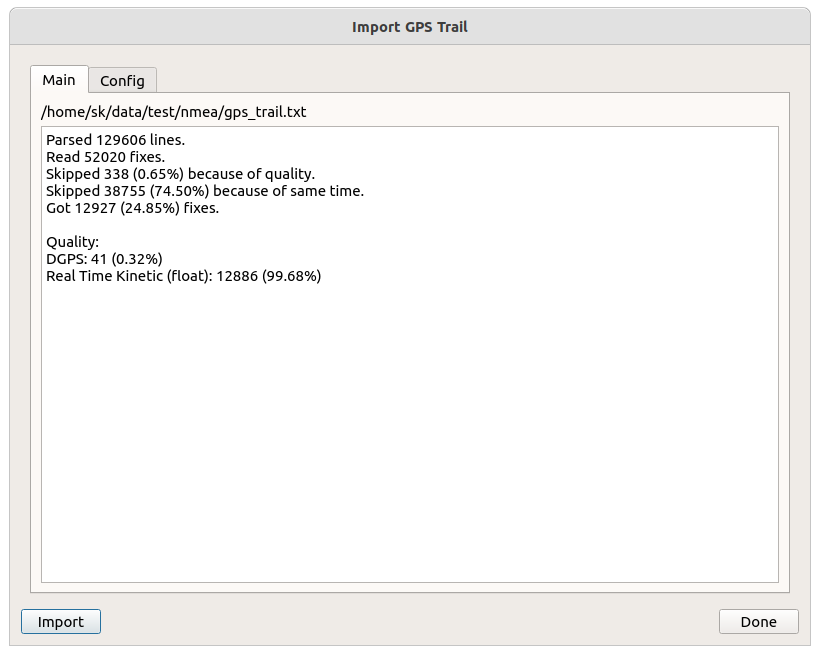
\includegraphics[width=16cm]{figures/gps_import_task.png}
  \caption{Import GPS Trail}
\end{figure}

There exist 2 tabs:

\begin{itemize}
\item Main: File path and information text
\item Config: Configuration of data source and secondary information
\end{itemize}
\ \\

\subsubsection{Main Tab}

At the top, a label exists indicating the file to be imported. \\

Below, a text field is given, which after selection of an NMEA file displays the content information and/or error messages. \\

\subsubsection{Config Tab}

\begin{figure}[H]
    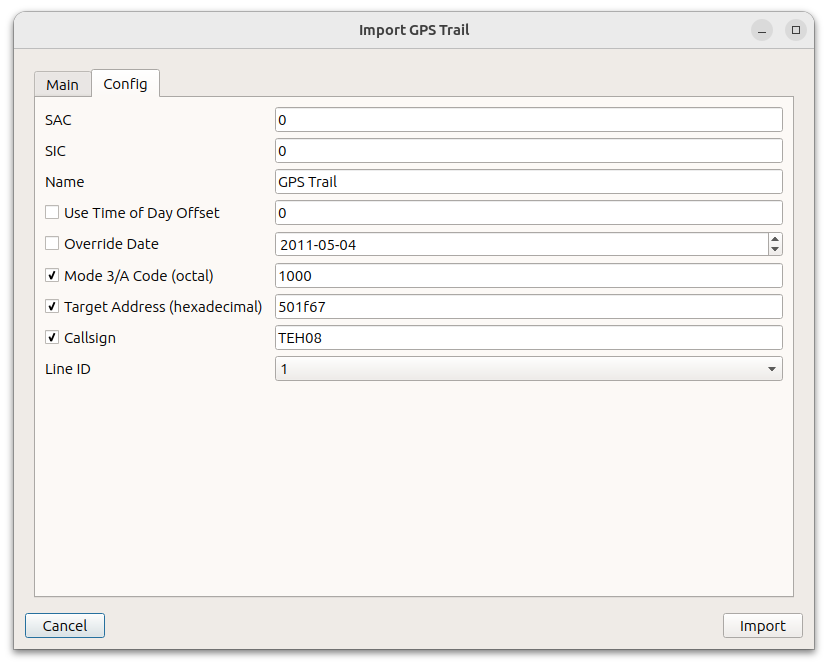
\includegraphics[width=16cm]{figures/gps_import_config.png}
  \caption{Import GPS Trail Config}
\end{figure}

In the configuration tab, several configuration parameters can be set:

\begin{itemize}
\item SAC: System area code of the reference data source
\item SIC: System identification code of the reference data source
\item Name: Name of the reference data source
\item Time of Day Offset: Time correction factor, in seconds. Set to 0 to disable.
\item Override Date: Set date information, e.g. if missing in NMEA file
\item Mode 3/A Code (octal): Mode 3/A code to be set. Uncheck checkbox to disable.
\item Target Address (hexadecimal): Mode S address to be set. Uncheck checkbox to disable.
\item Callsign: Target identification to be set. Uncheck checkbox to disable.
\item Line ID: Line to be used during import
\end{itemize}
\ \\

\subsubsection{Running}

After selecting an NMEA file, the task can be performed using the 'Import' button.

Please note that reference trajectory updates are skipped in the following two cases:
\begin{itemize}
\item The time is the same as the previous update
\item The quality is set to 0 (invalid position).
\end{itemize}
